\chapter{Evaluation}

\label{ch:eval}

\section{Training on Space Invaders}

Using the determined mutation and crossover operators, with the initial mr = 0.3, and cr = 0.35, the final set of models were trained. The CR is slightly decreased from the implementation chapter as this produces slightly better results. In this case, each agent had 14 episodes on the environment per generation, but the number of lives were still limited to 1. This reduced the training time, without too much of a deficit to the quality of the training.  This was tested for 25 generations, and the population contained 20 agents. The training curve can be seen in Fig. \ref{fig:final}, and how well the model performed compared to an agent which performed random action at each step for the Space Invaders game can be seen in Table \ref{ref:sptab}. To obtain these results both the best agent and the random agent had 14 episodes with the environment. We can see from this table that neuro-evolution with these parameters resulted in a 400\% increase in the score of the agent on Space Invaders, something which could increase with further training and a larger number of parameters in the model.

\begin{figure}[ht]
  \centering
  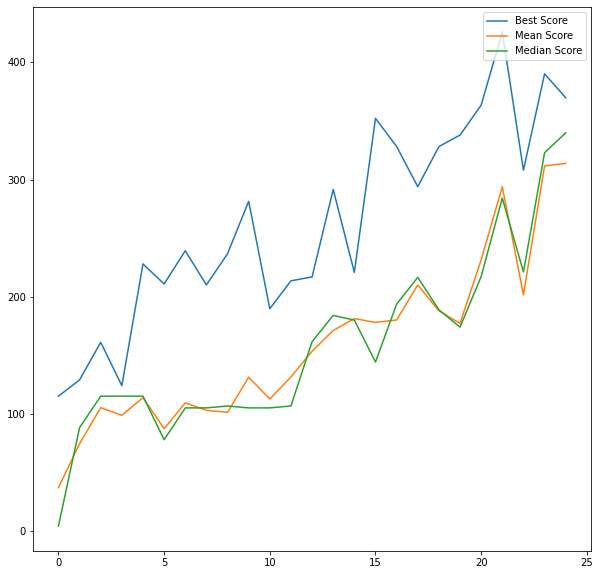
\includegraphics[scale=0.4]{images/final-run.png}
  \caption{Final Neuro-Evolution Training Graph (x-axis - current generation. y-axis - score)}
  \label{fig:final}
\end{figure}

\begin{table}[ht]
  \centering
  \begin{tabular}{| m{6cm} | r | r | r |}
    \hline
    \rowcolor{black!30} & Mean Score & Median Score & Best Score \\
    \hline
    Trained Agent Results & 552.0 & 625.0 & 670.0 \\
    \hline
    Random Action Agent Results & 153.0 & 155.0 & 205.0 \\
    \hline
  \end{tabular}
  \caption{Space Invaders - Trained Agent vs Random Action Agent}
  \label{ref:sptab}

\end{table}

\section{Transfer Learning}

The comparison between an agent performing random actions and the best agent taken from the final generation from the Space Invaders training for both new environments can be seen in Table. \ref{tab:dac}. Again, for both environments both the random agent and pre-trained agent experienced the environment 14 times. From these results we can say that utilising transfer learning for RL does not produce a significant improvement over using a random agent. In both Demon Attack and Carnival, the transfer learned agents did not perform better than a random agent at all. Whilst, in theory the agent should aim to shoot anything floating in the sky, perhaps the intricacies of the games were too different from Space Invaders. It is because of this that the DNN is unlikely to be able to utilise it's previously learnt knowledge to new environments. The initial question posed was \textbf{can we transfer the learning of DNNs trained with neuro-evolution techniques on one environment to another similar environment?} The answer is not with these environments. Space Invaders is too different from Carnival and Demon Attack, and in fact, a random agent outperformed the trained agent on the new environments, meaning that the transfer learning actually had an adverse affect.

\begin{table} [ht]
  \begin{tabular}{| m{8cm} | r | r | r |}
    \hline
    \rowcolor{black!30} & Mean Score & Median Score & Best Score \\
    \hline
    Demon Attack Random Agent & 181.786 & 175.0 & 385.0 \\
    \hline
    Demon Attack Pre-Trained Model & 83.2 & 70.0 & 235.0 \\
    \hline
    Carnival Random Agent & 717.1 & 690.0 & 1120 \\
    \hline
    Carnival Model Results & 410.0 & 410.0 & 620.0 \\
    \hline
  \end{tabular}
  \caption{Demon Attack and Carnival, Random vs Trained Agent Results}
  \label{tab:dac}
\end{table}
